\documentclass[a4paper,12pt]{article}

\usepackage{graphicx} % Required for inserting images
\usepackage{amsmath,amssymb,amsfonts}
\usepackage{subcaption}
% -----------------------
% Package Imports
% -----------------------

% Set page margins
\usepackage[a4paper, top=1in, bottom=0.8in, left=1.1in, right=0.8in]{geometry}

% Use Times New Roman font
\usepackage{times}

% Add page numbering
\pagestyle{plain}
\usepackage{multirow}
% Enable graphics inclusion
\usepackage{graphicx}
\usepackage{float}
% Enable code listings
\usepackage{listings}
\usepackage{xcolor} % For customizing code colors

% Define MATLAB style for listings
\lstdefinestyle{vscode-light}{
	language=Matlab,
	basicstyle=\ttfamily\footnotesize,
	keywordstyle=\color{blue},
	commentstyle=\color{gray},
	stringstyle=\color{red},
	numberstyle=\tiny\color{black},
	numbersep=5pt,
	frame=single,
	backgroundcolor=\color{white!10},
	breaklines=true,
	captionpos=b,
	tabsize=4,
	showstringspaces=false,
	numbers=left,  % Enable line numbering on the left
	stepnumber=1,  % Line numbers increment by 1
	numberfirstline=true, % Number the first line
}
\setlength{\parindent}{0pt}
\setlength{\parindent}{0pt}
\usepackage{sectsty}
\sectionfont{\fontsize{12}{15}\selectfont}


\begin{document}
	\textbf{Experiment No:} 2

\textbf{Name of the Experiment:} 
Design, Soldering and Testing of a Cell Phone Charger Circuit. \\
\textbf{Objective:}

	
	The objectives of this lab are:
	\begin{itemize}
		\item To study the operation and observe the AC to DC conversion using Bridge rectifier circuit.
		\item To Design and solder a Cell Phone Charger Circuit on PCB board .
		
		
	\end{itemize}

\section*{Theory:}

A Printed Circuit Board (PCB) is a crucial component in modern electronic systems, serving as a mechanical platform to electrically connect various components. The process of PCB design involves creating a blueprint of the electrical connections in a circuit and determining how components such as resistors, capacitors, diodes, and integrated circuits will be physically placed and connected. PCBs simplify complex wiring systems, reduce physical space requirements, and improve the durability of electronic devices.

A charger circuit is used to convert alternating current (AC) from a power supply into direct current (DC) to charge a battery or power electronic devices. The circuit typically steps down the high voltage from the mains to a lower, manageable DC voltage. A charger circuit converts high-voltage AC from mains to low-voltage DC for charging batteries or powering devices.

	
		\section*{Required Apparatus:}
	\begin{table}[H]
		\centering
		\caption{Components list for Astable Multivibrator}
		\begin{tabular}{|c|c|c|c|}
			\hline
			\textbf{\begin{tabular}[c]{@{}c@{}}SI \\ No.\end{tabular}} & \textbf{Components}                                                                   & \textbf{Specifications}                                                                     & \textbf{Quantity} \\ \hline
			1                                                          & PCB board                                                                             & \begin{tabular}[c]{@{}c@{}}Printed connection of\\    \\ astable multivibrator\end{tabular} & 1                 \\ \hline
			2                                                          & Resistor                                                                              &  1k$\Omega$                               & 2                 \\ \hline
			3                                                          & Capacitor                                                                             & \begin{tabular}[c]{@{}c@{}} 100µF polar \end{tabular}           & 2                 \\ \hline
			4                                                          & LED                                                                                   &                                                                                             & 1                 \\ \hline
			5                                                          & Transformer                                                                         &  \begin{tabular}[c]{@{}c@{}}220V - 50Hz \\    \\ 12Vx2, 1000mA\end{tabular}                                                                                    & 1                 \\ \hline
			6                                                          &  Diode                                                                             & 1N4007                & 4  \\ \hline
			7                                                          & 5V Voltage Regulator                                                                            & LM7805                                                                                         & 1                 \\ \hline
			8                                                          & Screw Connector                                                                          & 5mm                                                                           & 2                 \\ \hline
				9                                                          & \begin{tabular}[c]{@{}c@{}}2 pin Male-Female \\ Prong AC Power Cable Cord    \\ \end{tabular}                                                                          &            \begin{tabular}[c]{@{}c@{}}C8-Inlet,C7-Connector \\220V-2.5AMAX    \\ \end{tabular}                                                                    & 1                 \\ \hline
			10                                                          & \begin{tabular}[c]{@{}c@{}}Simulating and pcb\\    designing software\end{tabular} & KiCad 8.0                                                                                       &                   \\ \hline
		\end{tabular}
	\end{table}

	
	\section*{Circuit Diagram:}
	\begin{figure}[H]
		\centering
		\includegraphics[width=1\linewidth, height=.3\textheight]{"Images/6"}
		\caption{Schematic Diagram}
	\end{figure}
\vspace{2cm}
	
	
	\section*{Experimental Setup:}
		\begin{figure}[H]
		\centering
		\includegraphics[angle=270,width=1 \linewidth]{"Images/4"}
	
		\caption{Experimental Setup of cell phone charger}
	\end{figure}
	\newpage
\section*{Experimental Procedure:}

\begin{enumerate}
	\item Collected all necessary components including the PCB board, resistors, capacitors, transformer, diodes, voltage regulator, LED, and screw connectors.
	\item Designed the charger circuit using KiCad 8.0 software and generated the PCB layout.
	\item Assembled and placed all components on the PCB according to the circuit diagram.
	\item Soldered the components carefully, ensuring correct polarity for diodes, capacitors, and the voltage regulator (LM7805).
	\item Connected the transformer’s secondary output (12V x 2) to the input of the rectifier circuit made with diodes.
	\item Connected the output of the rectifier to the input of the voltage regulator (LM7805) to obtain a stable 5V DC output.
	\item Connected an LED at the output to indicate proper functioning and used screw connectors for easy input/output connections.
	\item Visually inspected the solder joints and verified circuit continuity using a multimeter.
	\item Connected the primary side of the transformer to 220V AC mains carefully.
	\item Measured the output voltage to ensure 5V DC was available and indicated RED LED which meant ready for charging a cell phone.
\end{enumerate}

	\section*{PCB Design:}
	\begin{figure}[H]
		\centering
		\includegraphics[width=0.51\linewidth]{"Images/7"}
		\caption{Schematic Diagram}
	\end{figure}
	\section*{Circuit diagram after soldering:}
	
	\begin{figure}[H]
		\centering
		\begin{subfigure}[t]{1\textwidth}
			\centering
			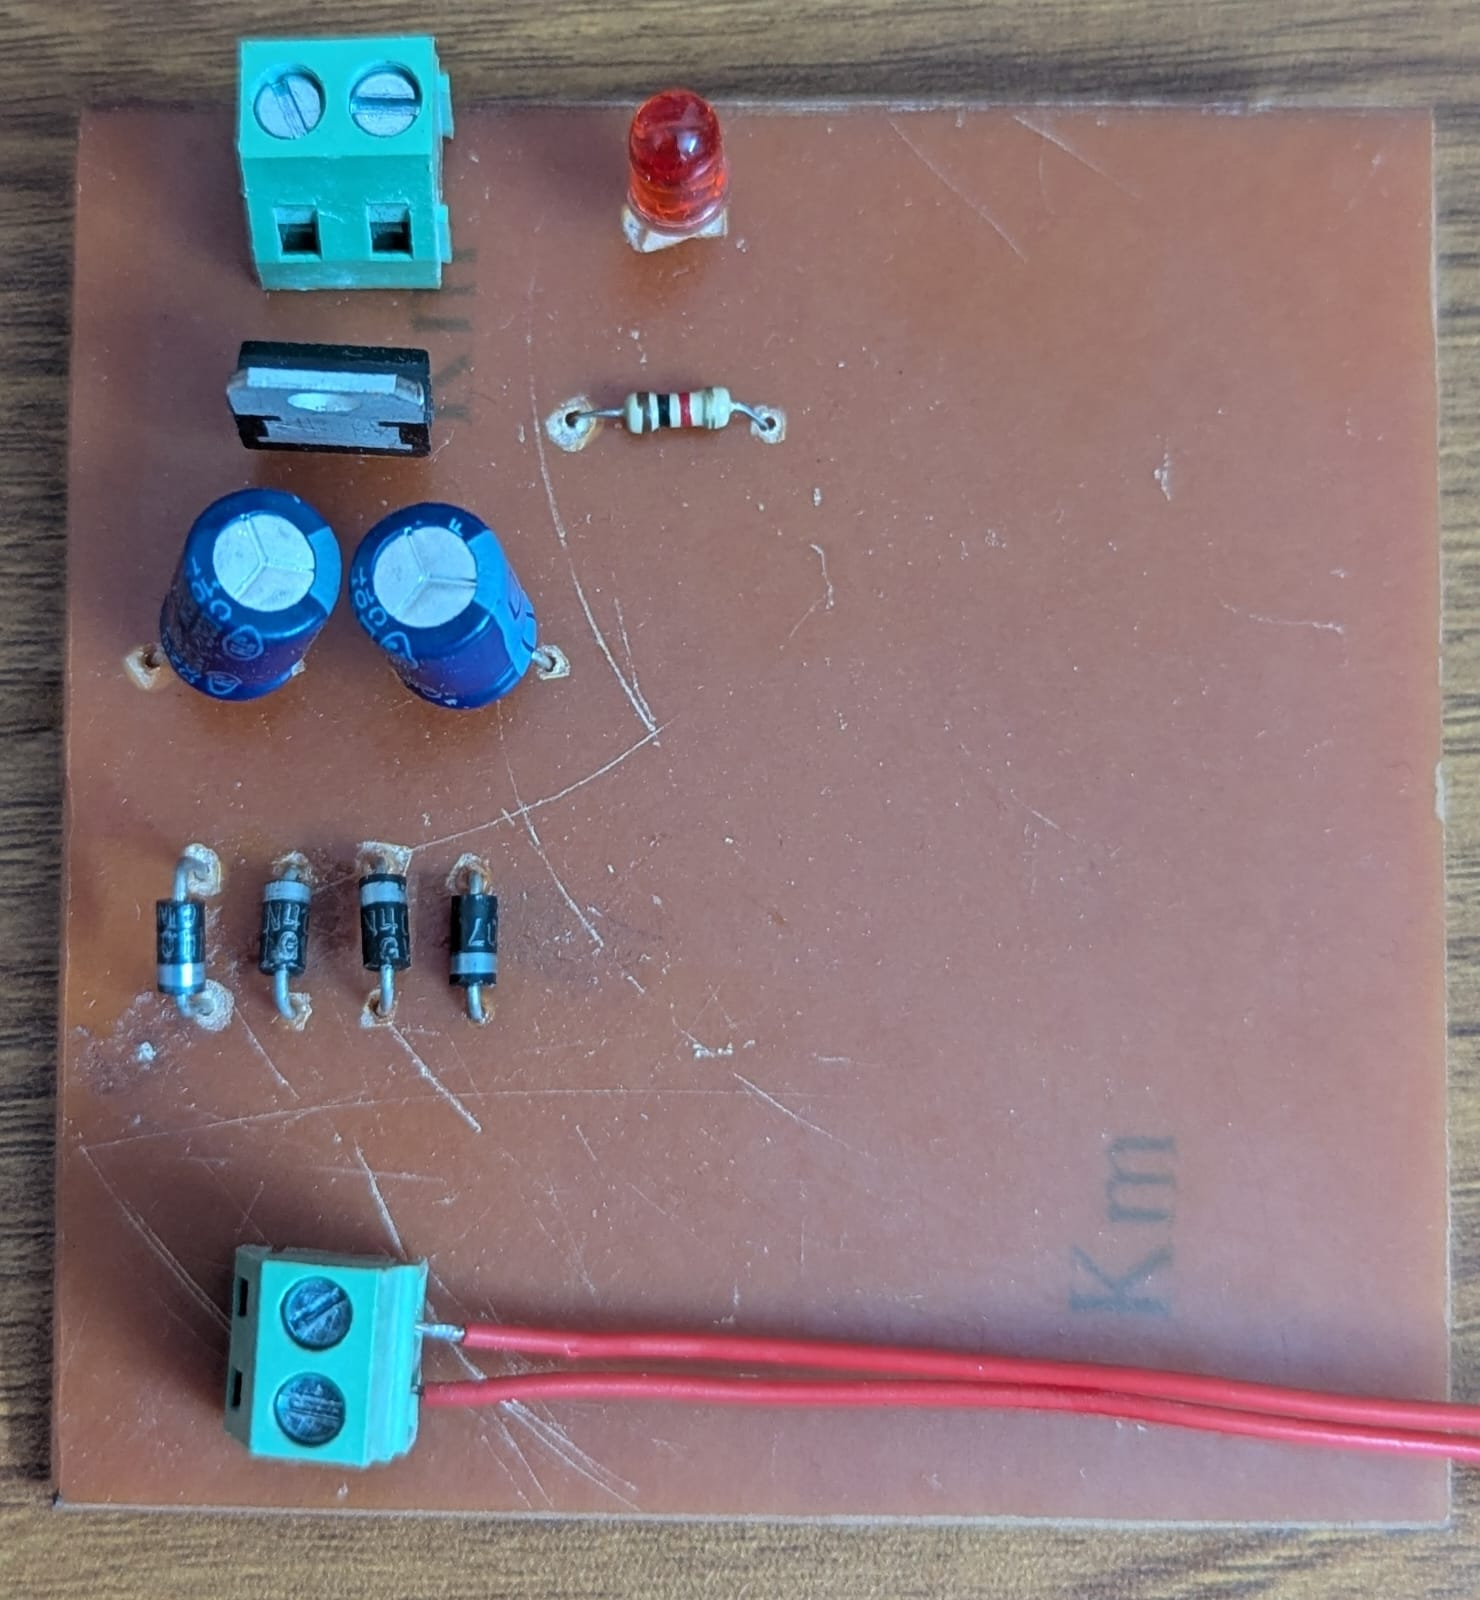
\includegraphics[width=0.5\linewidth]{Images/1}
			\caption{ Top side of the PCB board}
			\vspace{2cm}
		\end{subfigure}
		
		\begin{subfigure}[t]{1\textwidth}
			\centering
			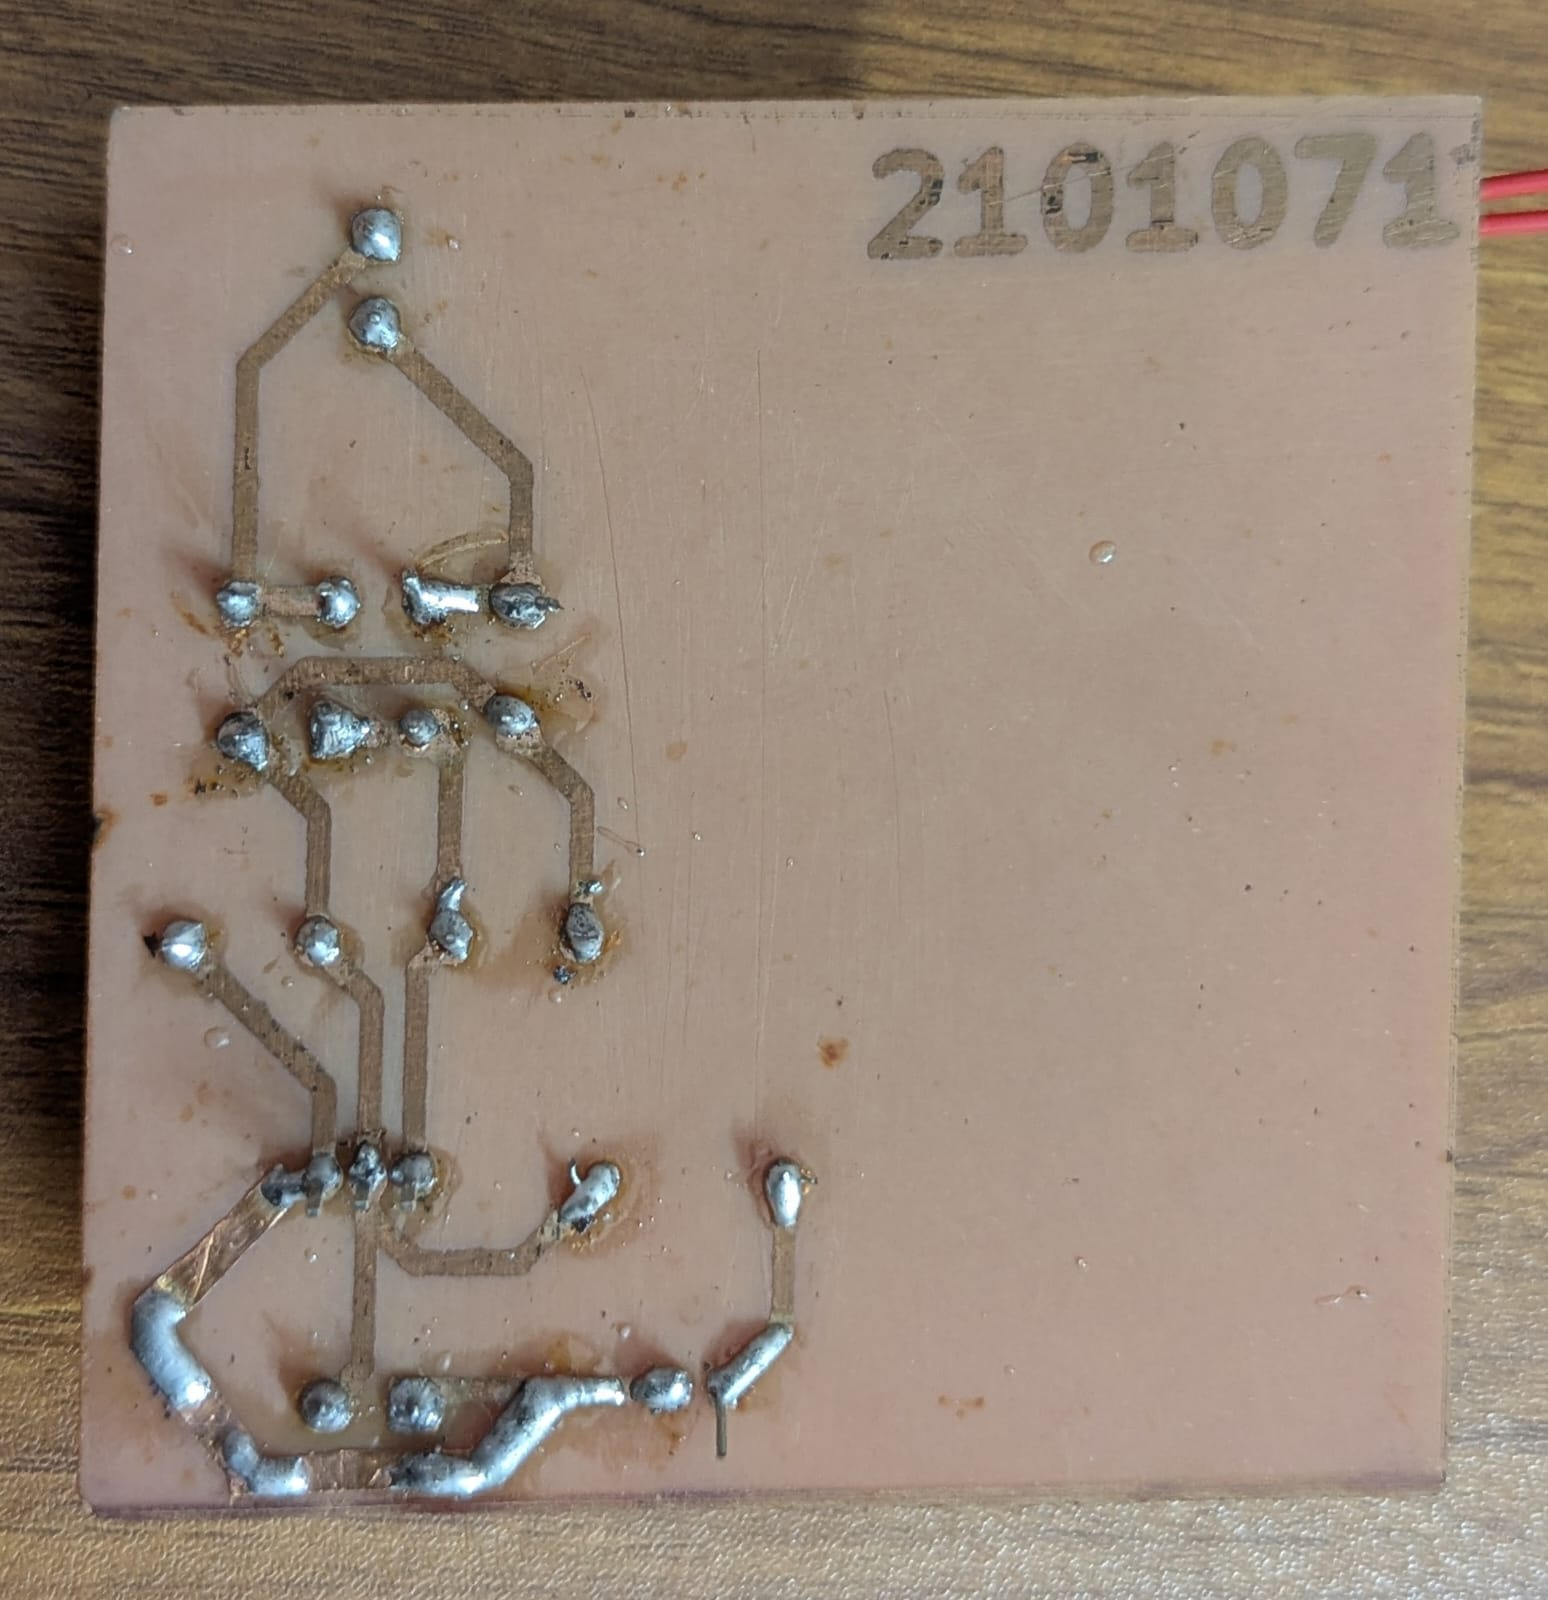
\includegraphics[width=0.5\linewidth]{Images/2}
			\caption{ Bottom side of the PCB board}
		\end{subfigure}
	\end{figure}
	
	\newpage
	\section*{Experimental Result:}
		\begin{figure}[H]
		\centering
		\includegraphics[width=0.44 \linewidth]{"Images/5"}
		
		\caption{Experimental result of cell phone charger}
	\end{figure}
	\section*{Discussion:}
	In the shop practice, we were given the task to design, solder, and test  a Cell Phone Charger Circuit using bridge rectifier circuit and voltage regulator IC.Throughout the experiment,The charger circuit was designed and soldered successfully on to the PCB board. To make the PCB board, the etching process was followed, where the PCB board was submerged in ferric chloride solution to make the desired tracing path. To place the components, holes were drilled. The components were placed and soldered onto the PCB with great care. To supply the board, a 220V AC voltage was used using 2pin AC power cable cord, which was connected to a screw connector. For a power indicator, an LED was placed to ensure the PCB's 5V power supply, which worked fine as power was supplied.
	\section*{Conclusion:}
	
	As the power supply was successfully connected and worked the power LED indicator, the circuit worked as expected.Though output voltage was about 4.954V in no load condition. The possible reasons for the PCB was not delivering the desired 5V output voltage could be faulty or loose solder joints,indicator LED's voltage drop,components or conducor's significant resistance which causes voltage drop. As there was no broken or shorted path and indicator LED was connected in parallel we can conclude that components or conductors's voltage drop after voltage regulation might be the possible and logical reason for showing slightly less from 5V.
	
	
\end{document}